\documentclass[12pt]{jarticle}
\usepackage{fancyhdr}
%\usepackage{jtygm}
\usepackage{amsmath}
\usepackage{amssymb}
\usepackage{graphicx}
\usepackage{braket}
\usepackage{color}
\usepackage{bm}% bold math
\usepackage{dcolumn}% Align table columns on decimal point

\topmargin=-10mm
\textheight=25cm
\textwidth=17cm
\oddsidemargin=-0.04 cm
\evensidemargin=-1.04cm

\begin{document}
%
% Cover
%
\title{FermiSurfer マニュアル \\
version 1.4}
\author{河村 光晶\footnote{mkawamura@issp.u-tokyo.ac.jp}}
%\date{}
\maketitle

\tableofcontents

\section{はじめに}

この文書ではFermi面描画ソフト「Fermi Surfer」についての解説を行っています. 
Fermi Surferは東京大学の河村光晶
が2012年頃から開発を行っていたもので, 
2014年11月に公開されました. 
Fermi面を描画しその上に各種物理量(超伝導ギャップ関数や軌道キャラクターなど)
をカラープロットするソフトウェアです. 

\section{MIT ライセンス}

Copyright (c) 2014 Mitsuaki Kawamura

\vspace{0.5cm}
以下に定める条件に従い、
本ソフトウェアおよび関連文書のファイル(以下「ソフトウェア」)の複製を取得するすべての人に対し、
ソフトウェアを無制限に扱うことを無償で許可します。
これには、ソフトウェアの複製を使用、複写、変更、結合、掲載、頒布、サブライセンス、
および/または販売する権利、およびソフトウェアを提供する相手に同じことを許可する権利も無制限に含まれます。

\vspace{0.5cm}
上記の著作権表示および本許諾表示を、ソフトウェアのすべての複製または重要な部分に記載するものとします。

\vspace{0.5cm}
ソフトウェアは「現状のまま」で、明示であるか暗黙であるかを問わず、何らの保証もなく提供されます。
ここでいう保証とは、商品性、特定の目的への適合性、および権利非侵害についての保証も含みますが、
それに限定されるものではありません。 作者または著作権者は、契約行為、不法行為、またはそれ以外であろうと、
ソフトウェアに起因または関連し、あるいはソフトウェアの使用またはその他の扱いによって生じる一切の請求、損害、
その他の義務について何らの責任も負わないものとします。 

\section{このパッケージに含まれているファイル}
\begin{description}
\item[\texttt{bin/fermisurfer.exe}] Windows用実行ファイル
\item[\texttt{doc/manual\_en.pdf}] マニュアル(英語)
\item[\texttt{doc/manual\_ja.pdf}] マニュアル(日本語)
\item[\texttt{examples/mgb2\_vfz.frmsf}] サンプル入力ファイル
\item[\texttt{src/fermisurfer.c}] ソースファイル
\item[\texttt{src/mac.diff}] Mac OSX用 パッチ
\item[\texttt{src/Makefile}] Linux用 Makefile
\item[\texttt{src/Makefile-mac}] Mac OSX用 Makefile
\end{description}

\section{インストール手順}

\subsection{Linuxの場合}

\begin{enumerate}

\item 必要なパッケージをインストール(既にパッケージが入っている場合は何も起こりません. )

  \begin{itemize}
  \item Debian/Ubuntu 等
    \begin{verbatim}
    $ sudo aptitude install freeglut3-dev
    \end{verbatim}
  \item Red Hat Enterprise Linux/CentOS 等
    \begin{verbatim}
    $ sudo yum install freeglut-devel.x86_64
    \end{verbatim}
  \end{itemize}

\item メイク

\begin{verbatim}
  $ cd ./src
  $ make fermisurfer
  $ make install
\end{verbatim}

\end{enumerate}

以上で実行可能ファイル \texttt{fermisurfer} が作られ、\verb|/usr/local/bin/|にコピーされます.

\subsection{Mac OSX の場合}

\begin{enumerate}

\item Xcodeをあらかじめインストールしておく
\item ソースコードにパッチを当てる
\begin{verbatim}
  $ cd ./src
  $ patch -p1 < mac.diff
\end{verbatim}

\item メイク
\begin{verbatim}
  $ make -f Makefile-mac fermisurfer
  $ make -f Makefile-mac install
\end{verbatim}

\end{enumerate}

以上で実行可能ファイル \texttt{fermisurfer} が作られ、\verb|/usr/local/bin/|にコピーされます.

\subsection{Windowsの場合}

\begin{enumerate}

\item freeglutWindows Development Libraryのサイト
\begin{verbatim}
http://www.transmissionzero.co.uk/software/freeglut-devel/
\end{verbatim}
内の「freeglut MSVC package」という項目から
\texttt{freeglut.dll}を含む\texttt{zip}ファイルを
ダウンロードし, 展開する.

\item 展開したフォルダ内の\texttt{bin}というフォルダに入っている,
\texttt{freeglut.dll}を\texttt{fermisurfer.exe}のあるフォルダ(\verb|bin|)にコピーする.

(注) \verb|bin\x64\|にも\verb|freeglut.dll|があるが, そちらは使わない.

\item \verb|fermisurfer.exe|と\verb|freeglut.dll|は常に同じフォルダにおいておくこと.

\end{enumerate}

\section{Input file}

\subsection{input fileの書式}

用意するデータは, 
\begin{itemize}
\item Brillouin領域分割数(3方向)
\item 逆格子ベクトル
\item バンド本数
\item 軌道固有値(以下エネルギーと呼びます)の各バンド, $k$グリッド点での値
\item カラープロットしたい物理量(以下物理量と呼びます)の各バンド, $k$グリッド点での値
\end{itemize}
です. 

※ $k$グリッドの取り方
$k$点の取り方として, ${\rm \Gamma}$点を含むグリッドと, 
${\rm \Gamma}$点から半グリッド分だけずらしたグリッドの二つに対応しています(図1). 
後者はプロットしたい物理量が${\rm \Gamma}$点で特異的になっている
場合等に使われる事を想定しています. 

上記データを次のとおりの書式で並べます(サンプルファイル \verb|mgb2_vfz.frmsf|の中身). 

\begin{verbatim}
          40          40          36         (1)
           0                                 (2)
           3                                 (3)
   1.0000000      0.57735026      -0.0000000 (4)
   0.0000000       1.1547005       0.0000000 (5)
   0.0000000      -0.0000000      0.87206507 (6)
  2.91340202E-02                             (7)
  2.93242838E-02
  2.98905596E-02
  3.08193434E-02
     :
     :
  0.14393796
  0.12800488
  0.0000000                                  (8)
  0.36269817
  0.71675694
  1.0535113
  1.3644149
     :
     :
  -26.409407
  -19.318560
  -10.315671
\end{verbatim}

\begin{enumerate}
  \renewcommand{\labelenumi}{(\arabic{enumi})}
  \item $k$グリッド数
  \item ${\rm \Gamma}$点を含むグリッド(含まないグリッドでは1とする)
  \item バンド本数
  \item 逆格子ベクトル1 (任意単位)
  \item 逆格子ベクトル2
  \item 逆格子ベクトル3
  \item エネルギー (並び順は下記参照)
  \item 物理量 (並び順は下記参照)
\end{enumerate}

\subsection{C, fortranでの入力ファイルの書き出し方}

・fortran

\begin{verbatim}
  real(4) :: bvec1(3), bvec2(3), bvec3(3) !逆格子ベクトル
  integer :: nk1, nk2, nk3 !各逆格子ベクトルの方向の分割数
  integer :: ishift !グリットをシフトさせるか(=1)否か(=0)
  integer :: nbnd !バンド数
  real(4) :: eig(nk3,nk2,nk1,nbnd) !エネルギー
  real(4) :: x(nk3,nk2,nk1,nbnd) !物理量

  integer :: ik1, ik2, ik3, ibnd, fo

  open(fo, file = “sample.frmsf”)
  write(fo,*) nk1, nk2, nk3
  write(fo,*) ishift
  write(fo,*) nbnd
  write(fo,*) real(bvec1(1:3))
  write(fo,*) real(bvec2(1:3))
  write(fo,*) real(bvec3(1:3))
  do ibnd = 1, nbnd
     do ik1 = 1, nk1
        do ik2 = 1, nk2
           do ik3 = 1, nk3
              write(fo,*) real(eig(ik3,ik2,ik1,ibnd)) 
           end do
        end do
     end do
  end do
  do ibnd = 1, nbnd
     do ik1 = 1, nk1
        do ik2 = 1, nk2
           do ik3 = 1, nk3
              write(fo,*) real(x(ik3,ik2,ik1,ibnd)) 
           end do
        end do
     end do
  end do
  close(fo)
\end{verbatim}

・C言語

\begin{verbatim}
  float bvec1[3], bvec2[3], bvec3[3]; /*逆格子ベクトル*/
  int nk1, nk2, nk3; /*各逆格子ベクトルの方向の分割数*/
  int ishift; /*グリットをシフトさせるか(=1)否か(=0)*/
  int nbnd; /*バンド数*/
  float eig[nbnd][nk1][nk2][nk3]; /*エネルギー*/
  float x[nbnd][nk1][nk2][nk3]; /*物理量*/

  FILE* fo;
  int ibnd, ik1, ik2, ik3;

  fo = fopen(“sample.frmsf”, “w”);
  ierr = fprintf(fo, "%d %d %d", nk1, nk2, nk3);
  ierr = fprintf(fo, "%d, iswitch);
  ierr = fprintf(fo, "%d, nbnd);
  ierr = fprintf(fp, "%e %e %e", bvec1[0], bvec1[1], bvec1[2]); 
  ierr = fprintf(fp, "%e %e %e", bvec2[0], bvec2[1], bvec2[2]);
  ierr = fprintf(fp, "%e %e %e", bvec3[0], bvec3[1], bvec3[2]);
  for (ibnd = 0; ibnd < nbnd; ++ibnd) {  
    for (ik1 = 0; ik1 < nk1; ++ik1) { 
      for (ik2 = 0; ik2 < nk2; ++ik2) { 
        for (ik3 = 0; ik3 < nk3; ++ik3) { 
          ierr = fprintf(fo, "%e", eig[ibnd][ik1][ik2][ik3]); 
        } 
      } 
    } 
  } 
  for (ibnd = 0; ibnd < nbnd; ++ibnd) {  
    for (ik1 = 0; ik1 < nk1; ++ik1) { 
      for (ik2 = 0; ik2 < nk2; ++ik2) { 
        for (ik3 = 0; ik3 < nk3; ++ik3) { 
          ierr = fprintf(fo, "%e", x[ibnd][ik1][ik2][ik3]); 
        } 
      } 
    } 
  } 
  fclose(fo); 
\end{verbatim}

\section{操作方法}

\subsection{Linuxの場合}
作成した実行可能ファイル\verb|fermisurfer|にパスが通っている状態で
\begin{verbatim}
$ fermisurfer mgb2_vfz.frmsf
\end{verbatim}
とコマンド, スペース, 入力ファイル名とタイプします. 
(サンプルファイルの中身はMgB$_2$のFermi速度の$z$方向成分です. )

\subsection{Windowsの場合}

入力ファイル(この場合は\verb|mgb2_vfz.frmsf|)を右クリックし,
メニューから「プログラムから開く」を選択し,
実行ファイルを\verb|fermisurfer.exe|に設定してください.

\vspace{0.5cm}
このあとはLinux, Windows共通です.
\verb|fermisurfer|が起動すると,
まずファイルから読み取った情報が出力されます. 

\begin{verbatim}
#####  Brillouin zone informations  ##### 

k point grid : 40 40 36 
k point grid is not shifted 
# of bands : 3 
bvec 1 : 1.000000 0.577350 -0.000000 
bvec 2 : 0.000000 1.154701 0.000000 
bvec 3 : 0.000000 -0.000000 0.872065 

# of lines for BZ : 84  (1)

#####  Max. and Min. of each bands  ##### 
     
Band   Eig_Min.      Eig_Max      Mat_Min      Mat_Max 
1     -0.428153     0.056262     -24.048639     24.048639 (2)
2     -0.289572     0.121181     -23.320309     23.320309 (2)
3     -0.133566     0.497620     -43.651634     43.651634 (2)

#####  First Brillouin zone mode  #####

band   # of patchs
1       8824  (3)
2       29469 (3)
3       28315 (3)

band   # of nodeline 
1       632   (4)
2       1524  (4)
3       2268  (4)

#####  Full color scale  ##### 

Max. value : 22.283419  (5)
Min. value : -22.283419 (5) 

\end{verbatim}

\begin{enumerate}
  \renewcommand{\labelenumi}{(\arabic{enumi})}
  \item Brillouin領域の境界を表示する線の数.
  \item それぞれのバンドにおけるエネルギーと物理量の最小値・最大値.
  \item それぞれのバンドにおけるパッチ(Fermi面を構成する平面)の数.
  \item それぞれのバンドにおけるnode line (後述)の本数.
  \item 物理量のFermi面における最大値と最小値.
    この数字がカラーバーの最大・最小に対応します. 
    下の例では一番青いところが-22.283419, 一番赤いところが22.283419となります.
    (2)で表示されているのはBrillouin領域全体のものです.    
\end{enumerate}

次に操作方法が出力され, Fermi面が描画されます. 

\begin{figure}[!ht]
  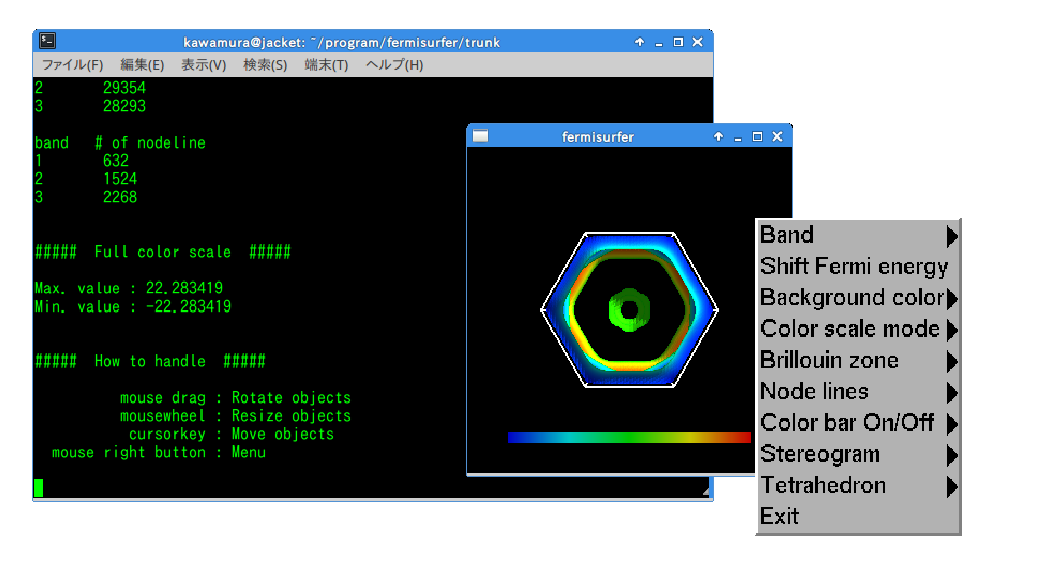
\includegraphics[width=17cm]{figs/start.eps}
  \caption{Fermisurferを起動した直後の画面.}
  \label{fig_start}
\end{figure}

\begin{itemize}
\item マウスのドラッグによる回転が出来ます. 
\item マウスのホイールを使っての拡大・縮小が出来ます. 
\item ウィンドウの大きさを変えることもできます. 
\item カーソルキーを使ってウィンドウ内で上下左右に図を動かせます. 
\item ウィンドウ内でマウスの右クリックをするとメニューが表示されます. 
\end{itemize}

次から右クリックで表示されるメニューを説明します. 

\subsection{Band}

バンド毎の表示on/offを切り替えます(図\ref{fig_band}).

\begin{figure}[!ht]
  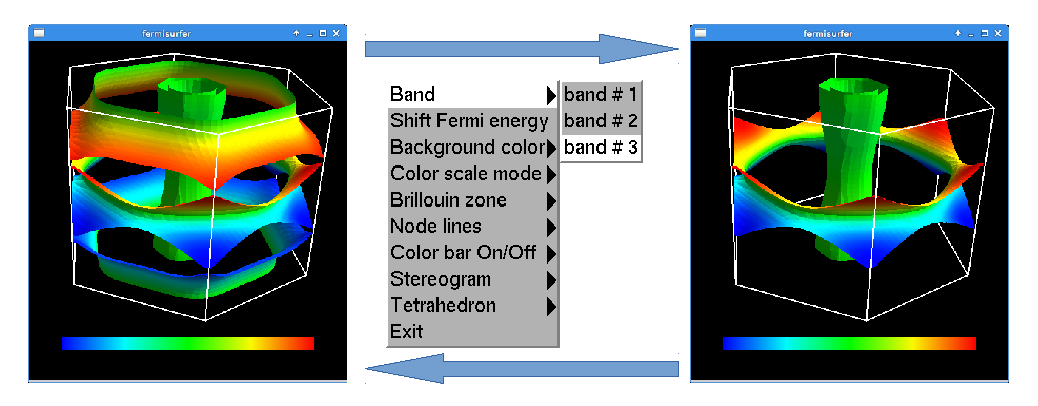
\includegraphics[width=17cm]{figs/band.eps}
  \caption{\texttt{Band} メニューで3番目のバンドの表示/非表示を切り替える.}
  \label{fig_band}
\end{figure}

\subsection{Mouse Drag}

マウスの左ボタンドラッグを行った時の動作を変更します.

\begin{description}
\item[Rotate(デフォルト)] ドラッグをした方向に図形を回転させます.
\item[Scale] 上方にドラッグすると図形を拡大, 下方にドラッグすると図形を縮小します.
\item[Translate] ドラッグした方向に図形を動かします.
\end{description}

\subsection{Shift Fermi energy}

Fermiエネルギー(デフォルトでは0)を任意の値にずらします.
このメニューを選択すると次のようにインプット中の最小のエネルギー, 
最大のエネルギー, 
現在のFermiエネルギーが標準出力として表示されます. 
\begin{verbatim}
Min  Max  E_F 
-0.428153 0.497620 0.000000 
Fermi energy shift : 
\end{verbatim}
次に新しいFermiエネルギーを入力すると, 
Fermi面が再描画されます (図\ref{fig_shift}).

\begin{figure}[!ht]
  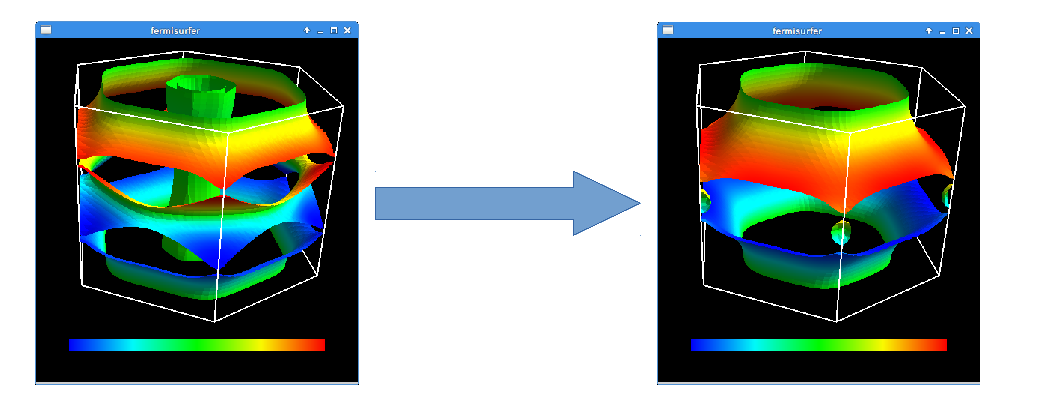
\includegraphics[width=17cm]{figs/shift.eps}
  \caption{\texttt{Shift Fermi energy}メニューで
    Fermi エネルギーを0 Ryから0.1 Ryに変える.}
  \label{fig_shift}
\end{figure}

\subsection{Background color}

背景色を黒または白に切り替えます. 
Brillouin Zoneの枠線も白/黒と切り替わります (図\ref{fig_background}). 

\begin{figure}[!ht]
  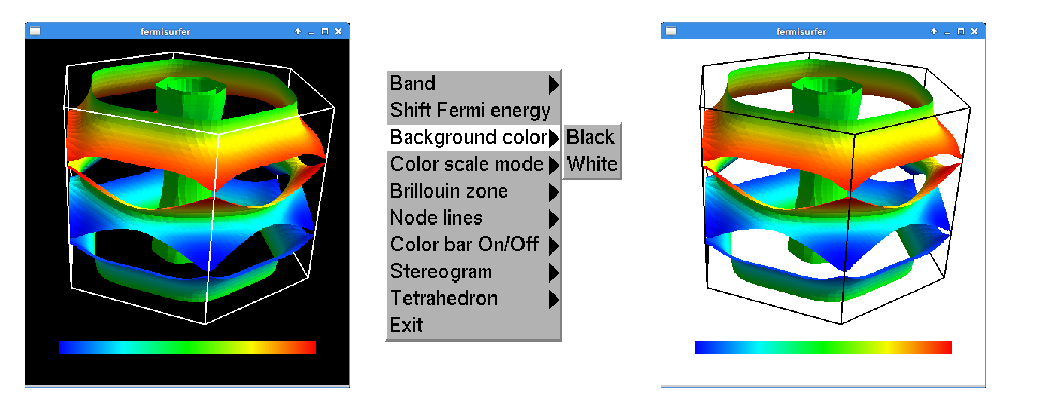
\includegraphics[width=17cm]{figs/background.eps}
  \caption{\texttt{Background color}メニューで背景色を白/黒に切り替える.}
  \label{fig_background}
\end{figure}

\subsection{Color scale mode}

Fermi面の色表示のさせ方を変更します(図\ref{fig_colorscale}). 
\begin{description}
\item[Auto(デフォルト)] 
  カラースケールの範囲をFermi面上での物理量の最小値から最大値までとします.
\item[Manual] カラースケールの範囲を標準入力から設定します.
\item[Unicolor] 物理量に関係なく, 各バンド毎に単色でFermi面を塗ります.
\item[Periodic] 周期的な量のプロットに用います。
  物理量が
  0 $\rightarrow$ $\pi/3$ $\rightarrow$ $2\pi/3$ $\rightarrow$ $\pi$ $\rightarrow$ 
  $4\pi/3$ $\rightarrow$ $5\pi/3$ $\rightarrow$ $2\pi$
  と変化するに連れて色が
  赤$\rightarrow$黄$\rightarrow$緑$\rightarrow$シアン$\rightarrow$青$\rightarrow$
  マゼンタ$\rightarrow$赤と変わります. 
\end{description}

\begin{figure}[!ht]
  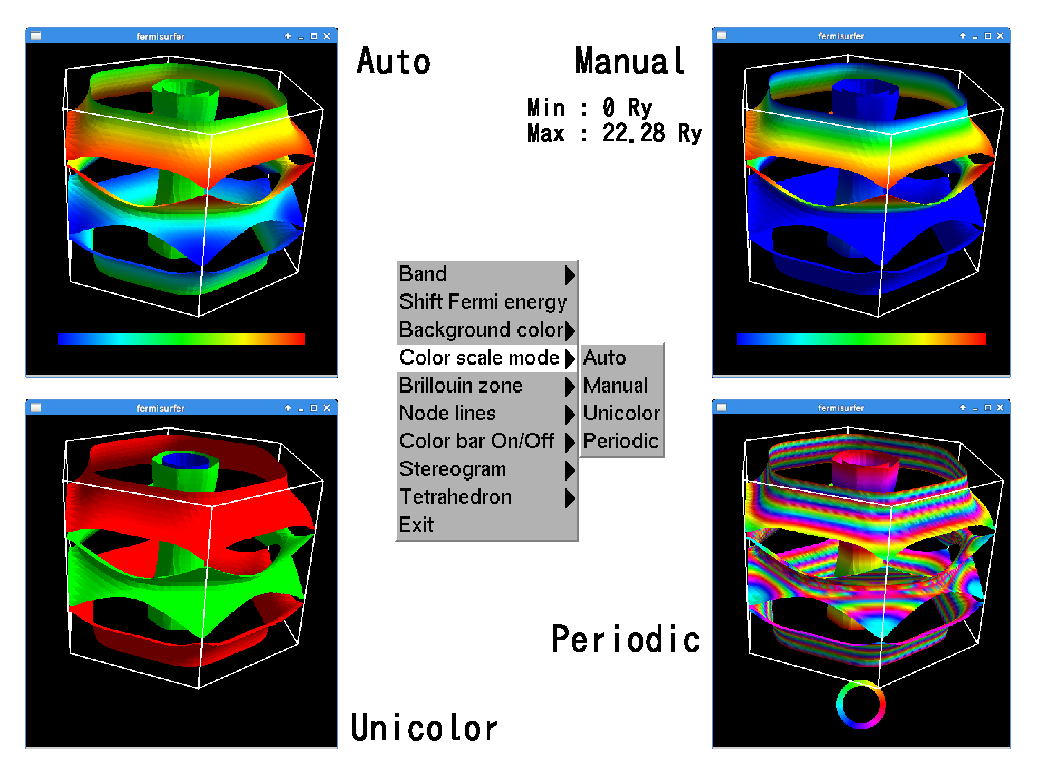
\includegraphics[width=17cm]{figs/colorscale.eps}
  \caption{\texttt{Color scale mode}メニュー.}
  \label{fig_colorscale}
\end{figure}

\subsection{Brillouin zone}

描画範囲をFirst Brillouin Zone/Primitive Brillouin Zoneと切り替える事が出来ます
(図\ref{fig_brillouinzone}).
\begin{description}
\item[Fisrst Brillouin Zone] ${\rm \Gamma}$ 点から一番近いBragg面で囲まれた領域
\item[Primitive Brillouine Zone] 逆格子ベクトルを辺とする平行6面体領域
\end{description}

\begin{figure}[!ht]
  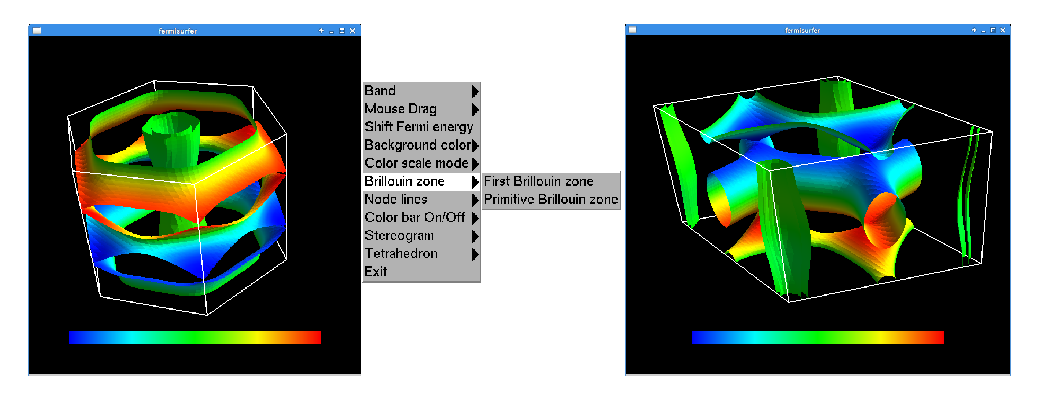
\includegraphics[width=17cm]{figs/brillouinzone.eps}
  \caption{\texttt{Brillouin zone} メニューでBrillouin領域のとり方を変更する.}
  \label{fig_brillouinzone}
\end{figure}

\subsection{Node line}

物理量が0となるところに引く線(node line)のOn/Offを切り替えます(図\ref{fig_nodeline}).

\begin{figure}[!ht]
  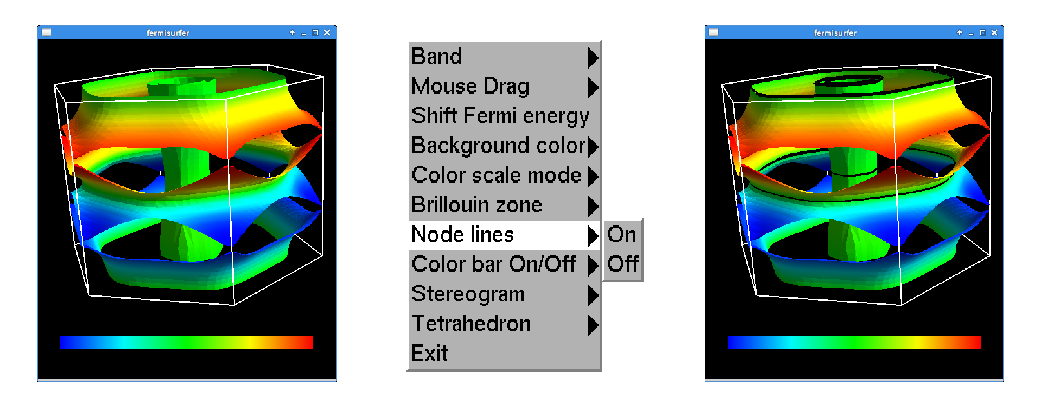
\includegraphics[width=17cm]{figs/nodeline.eps}
  \caption{\texttt{Node line} メニューでnode lineの表示/非表示を切り替える.}
  \label{fig_nodeline}
\end{figure}

\subsection{Color bar On/Off}

カラーバーの表示/非表示を切り替えます(図 \ref{fig_colorbar}). 

\begin{figure}[!ht]
  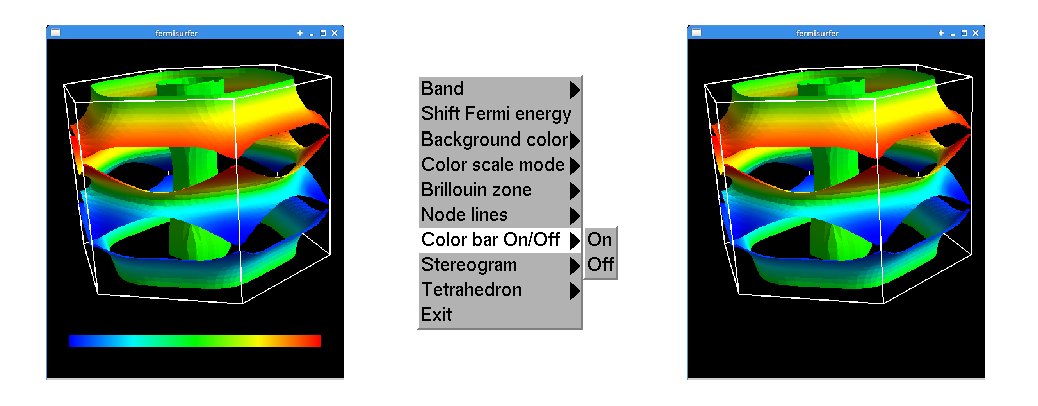
\includegraphics[width=17cm]{figs/colorbar.eps}
  \caption{\texttt{Color bar On/Off}メニューでカラーバーの表示/非表示を切り替える.}
  \label{fig_colorbar}
\end{figure}

\subsection{Stereogram}

裸眼立体視用の図の表示/非表示を切り替えます(図 \ref{fig_stereogram}). 
\begin{description}
\item[None (デフォルト)] 立体視を無効にします. 
\item[Parallel] 平行法用の図を表示します. 
\item[Cross] 交差法用の図を表示します. 
\end{description}

\begin{figure}[!ht]
  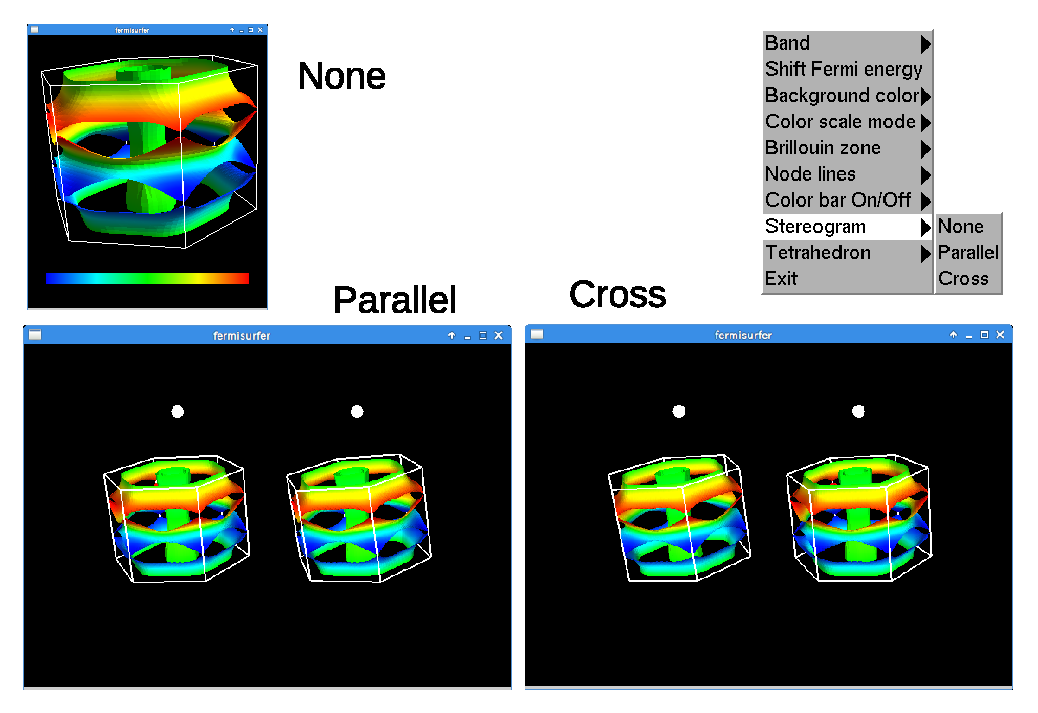
\includegraphics[width=17cm]{figs/stereogram.eps}
  \caption{\texttt{Stereogram} メニューで立体視用画像を表示する.}
  \label{fig_stereogram}
\end{figure}

\subsection{Tetrahedron}

四面体の切り方を変えます(デフォルトは\texttt{tetra \# 1}).
図が綺麗になる可能性がありますが, 
多くの場合は逆に図がギザギザして汚くなるようです. 

\subsection{Exit}

Fermi Surferを終了します. 

\section{ギャラリー}

IrO$_2$のHall係数に対するFermi面上の各軌道からの寄与
(Fig. \ref{fig_iro2}. 理化学研究所 有田グループ 佐野航氏提供). 

\begin{figure}[!ht]
  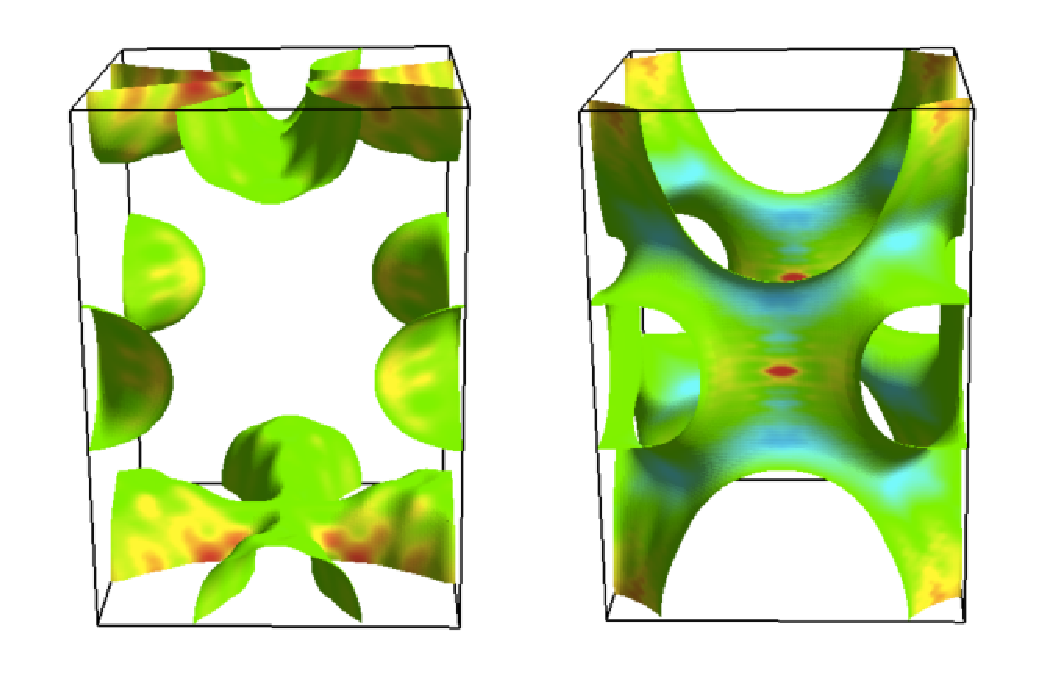
\includegraphics[width=17cm]{figs/iro2.eps}
  \caption{IrO$_2$のHall係数に対するFermi面上の各軌道からの寄与.}
  \label{fig_iro2}
\end{figure}

\section{謝辞}

東京大学物性研究所 小西優祐氏には, Mac OSXでの動作チェックおよびMakefile, 
パッチの提供をしていただいたことに感謝する.

\section{問い合わせ先}

プログラムのバグや質問は以下のフォーラムへご投稿ください.
\begin{verbatim}
http://sourceforge.jp/projects/fermisurfer/forums/
\end{verbatim}

開発に参加したい方は以下の連絡先にて受け付けております. 

東京大学物性研究所

河村光晶

\verb|mkawamura@issp.u-tokyo.ac.jp|

\end{document}
